\section[\textit{The Wealth of Nations} (1776)]{\textit{An Inquiry into the Nature and Causes of the Wealth of Nations} (1776)}

    Adam Smith’s seminal work laid the foundations for classical economics. Its discussion on the division of labour, the invisible hand, and self-interest has influenced economic thought for centuries.

    \subsection[Of the Principle which gives occasion to the Division of Labour]{Book I, Chapter 2 \\
                \textit{Of the Principle which gives occasion to the Division of Labour}}

        \subsubsection{The invisible hand}

            \begin{quote}
                It is not from the benevolence of the butcher, the brewer, or the baker, that we expect our dinner, but from their regard to their own interest. We address ourselves, not to their humanity but to their self-love, and never talk to them of our own necessities but of their advantages.
            \end{quote}

            This famous passage introduces the idea that individuals acting out of self-interest—rather than from any altruistic impulse—unintentionally promote the public good. Smith’s “invisible hand” suggests that as each person seeks personal advantage, society as a whole benefits from the efficient allocation of resources.

        \subsubsection{Self-interest}

            \begin{quote}
                The Wealth of Nations is a stupendous palace erected upon the granite of self-interest.

                (George Stigler, “\textit{Smith’s Travels on the Ship of State}”, 1971)
            \end{quote}

            This metaphor underscores how self-interest is not merely a personal trait but the very bedrock of economic prosperity. The image of a palace built on self-interest conveys both the strength and the inevitability of individual pursuit in shaping markets and societal wealth.

        \subsubsection{Non-tuism}

            \begin{quote}
                The economic relation does not exclude from my mind everyone but me, it potentially includes everyone but you.
                
                (Wicksteed, "\textit{The Common Sense of Political Economy}", 1910)
            \end{quote}

            Though the term “non-tuism” is uncommon, this quote highlights that while individuals focus on their own interests, the effects of their actions extend beyond themselves. Even if we consciously attend only to our own benefit, our exchanges inevitably affect others, emphasizing the interconnected nature of economic relationships.

        \subsubsection{Exchange as a tug of war}

            \begin{figure}[h]
                \centering
                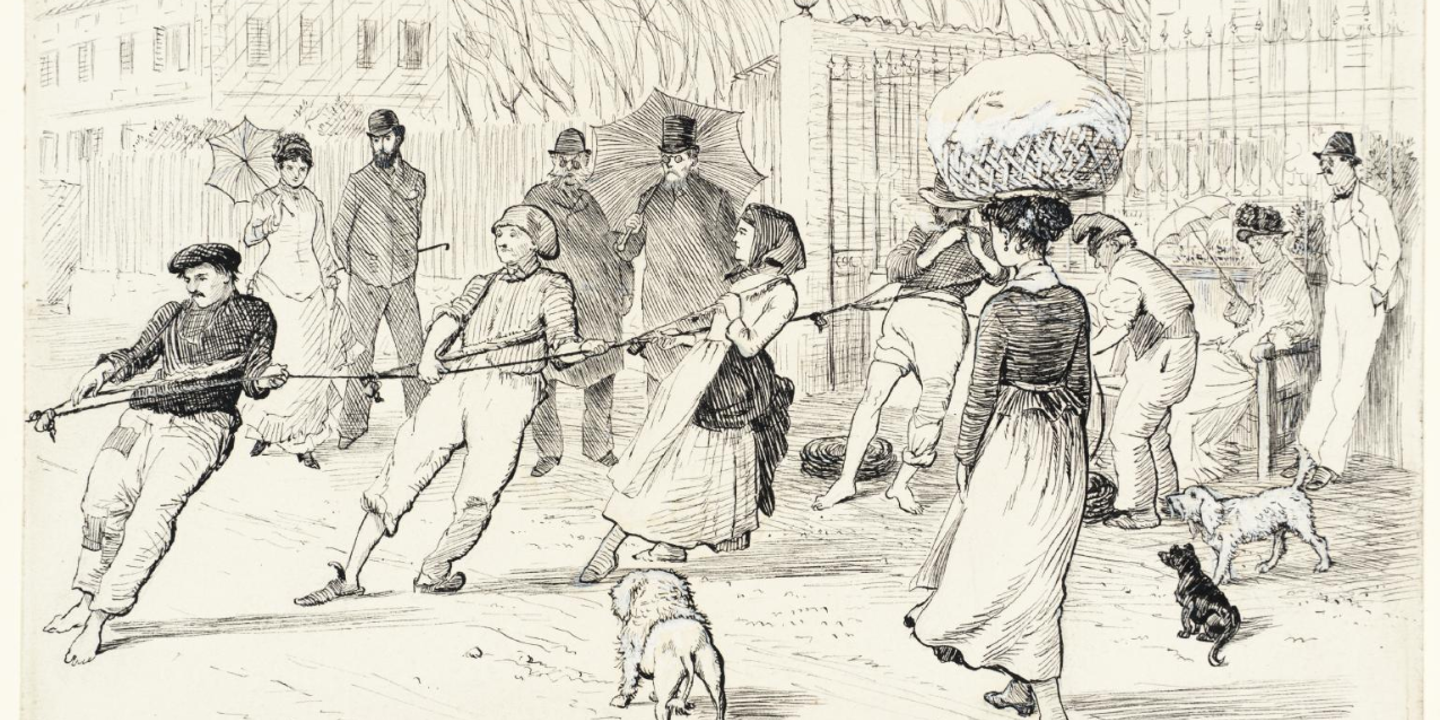
\includegraphics[width=0.5\linewidth]{Images/L6-1.png}
                \label{fig:L6-1}
            \end{figure}

    \subsection[Of the Division of Labour]{Book I, Chapter 1\\
                \textit{Of the Division of Labour}}

        \subsubsection{Advantages of the division of labour}

            \begin{quote}
                One man draws out the wire, another straights it, a third cuts it, a fourth points it, a fifth grinds it at the top for receiving the head…
            \end{quote}

            \begin{itemize}
                \item Increased worker dexterity
                \item Reduction of production time, eliminating the steps from one process to another
                \item Replacement of workers with machines
            \end{itemize}

            \begin{equation}
                \text{Division of Labour} \Rightarrow Exchange \xrightarrow{but \ in \ reality}{} Exchange \Rightarrow \text{Division of Labour}
            \end{equation}

    \subsection[Back to "Of the Principle which gives occasion to the Division of Labour"]{Back to Book I, Chapter 2 \\
                \textit{Of the Principle which gives occasion to the Division of Labour}}

        \subsubsection{The origin of division of labour}

            \begin{quote}
                This division of labour, from which so many advantages are derived, is not originally the effect of any human wisdom, which foresees and intends that general opulence to which it gives occasion. It is the necessary, though very slow and gradual consequence of a certain propensity in human nature which has in view no such extensive utility; the propensity to truck, barter, and exchange one thing for another.
            \end{quote}

        \subsubsection{Exchange in primitive society}

            \begin{quote}
                In a tribe of hunters or shepherds a particular person makes bows and arrows, for example, with more readiness and dexterity than any other. He frequently exchanges them for cattle or for venison with his companions; and he finds at last that he can in this manner get more cattle and venison, than if he himself went to the field to catch them. From a regard to his own interest, therefore, the making of bows and arrows grows to be his chief business, and he becomes a sort of armourer.

                Another excels in making the frames and covers of their little huts or moveable houses. He is accustomed to be of use in this way to his neighbours, who reward him in the same manner with cattle and with venison, till at last he finds it his interest to dedicate himself entirely to this employment, and to become a sort of house-carpenter.
            \end{quote}

    \subsection[That the Division of Labour is limited by the Extent of the Market]{Book I, Chapter 3 \\
                \textit{That the Division of Labour is limited by the Extent of the Market}}

        \subsubsection{No nailers in a small village}

            \begin{quote}
                It is impossible there should be such a trade as even that of a nailer in the remote and inland parts of the Highlands of Scotland. Such a workman at the rate of a thousand nails a day, and three hundred working days in the year, will make three hundred thousand nails in the year. But in such a situation it would be impossible to dispose of one thousand, that is, of one day's work in the year.
            \end{quote}

            \begin{figure}[h]
                \centering
                \includegraphics[width=0.75\linewidth]{Images/L6-2.png}
                \label{fig:L6-2}
            \end{figure}

    \subsection[Back to "Of the Principle which gives occasion to the Division of Labour"]{Back to Book I, Chapter 2 \\
                \textit{Of the Principle which gives occasion to the Division of Labour}}

        \subsubsection{Pursuit of one’s own interest that incidentally benefits that of others}

            \begin{quote}
                Two greyhounds, in running down the same hare, have sometimes the appearance of acting in some sort of concert. Each turns her towards his companion, or endeavours to intercept her when his companion turns her towards himself. This, however, is not the effect of any contract, but of the accidental concurrence of their passions in the same object at that particular time.
            \end{quote}

        \subsubsection{While we, the human beings}

            \begin{quote}
                We address ourselves, not to their humanity but to their \textit{self-love}, and never talk to them of our own necessities but of their advantages.
            \end{quote}

        \subsubsection{Self-interest?}

            \begin{quote}
                The Wealth of Nations is a stupendous palace erected upon the granite of self-interest.

                (George Stigler, “\textit{Smith’s Travels on the Ship of State}”, 1971)
            \end{quote} 

        \subsubsection{Egoism?}

            \begin{quote}
                Ce n’est pas de la bienveillance du boucher, du marchand de bière et du boulanger, que nous attendons notre dîner, mais bien du soin qu’ils apportent à leurs intérêts. Nous ne nous adressons pas à leur humanité, mais à leur égoïsme ; et ce n’est jamais de nos besoins que nous leur parlons, c’est toujours de leur avantage.

                (Translated by Germain Garnier, 1802)
            \end{quote}     

        \subsubsection{Fawning dogs}

            \begin{quote}
                When an animal wants to obtain something either of a man or of another animal, it has no other means of persuasion but to gain the favour of those whose service it requires. A puppy fawns upon its dam, and a spaniel endeavours by a thousand attractions to engage the attention of its master who is at dinner, when it wants to be fed by him.
            \end{quote}

        \subsubsection{We can’t all be friends}

            \begin{quote}
                Man sometimes uses the same arts with his brethren, and when he has no other means of engaging them to act according to his inclinations, endeavours by every servile and fawning attention to obtain their good will. He has not time, however, to do this upon every occasion. In civilized society he stands at all times in need of the cooperation and assistance of great multitudes, while his whole life is scarce sufficient to gain the friendship of a few persons.
            \end{quote}

        \subsubsection{Human beings exchange}

            \begin{quote}
                It is not from the benevolence of the butcher, the brewer, or the baker, that we expect our dinner, but from their regard to their own interest. We address ourselves, not to their humanity but to their self-love, and never talk to them of our own necessities but of their advantages.
            \end{quote}

        \subsubsection{The beggar}

            \begin{quote}
                Nobody but a beggar chuses to depend chiefly upon the benevolence of his fellow-citizens.
            \end{quote}

\section{\textit{The Theory of Moral Sentiments} (1759)}

    \subsection{The tightrope walker}

        \subsubsection{Sympathy}

            \begin{itemize}
                \item Immediate identification
                \item Without being a “passion contagion” (David Hume)
                \item Concordance, pleasure, approval
                \item Discordance, displeasure, disapproval
                \item Theory of moral judgment based on sentiments
            \end{itemize}

        \subsubsection{The impartial spectator}

            \begin{quote}
                When I endeavour to examine my own conduct, when I endeavour to pass sentence upon it, and either to approve or condemn it, it is evident that, in all such cases, I divide myself, as it were, into two persons; and that I, the examiner and judge, represent a different character from that other I, the person whose conduct is examined into and judged of. The first is the spectator, whose sentiments with regard to my own conduct I endeavour to enter into, by placing myself in his situation, and by considering how it would appear to me, when seen from that particular point of view. The second is the agent, the person whom I properly call myself, and of whose conduct, under the character of a spectator, I was endeavouring to form some opinion. The first is the judge; the second the person judged of.
            \end{quote}

            \begin{minipage}{0.48\textwidth}
                \begin{center}
                    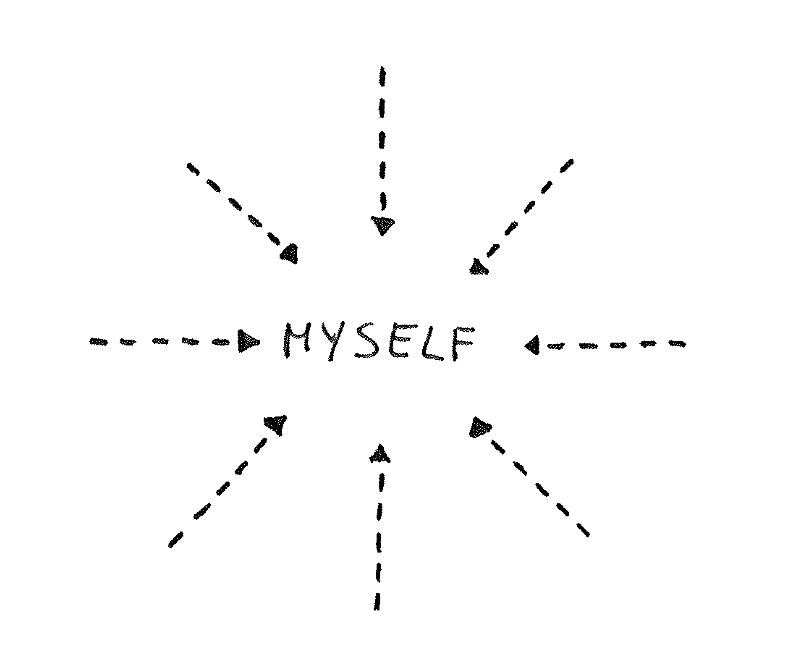
\includegraphics[width=1\linewidth]{L6-3a.png}
                    \captionof{figure}{Self-love as the pleasure of other’s approval}
                \end{center}
            \end{minipage}
            \begin{minipage}{0.04\textwidth}
                
            \end{minipage}
            \begin{minipage}{0.48\textwidth}
                \begin{center}
                    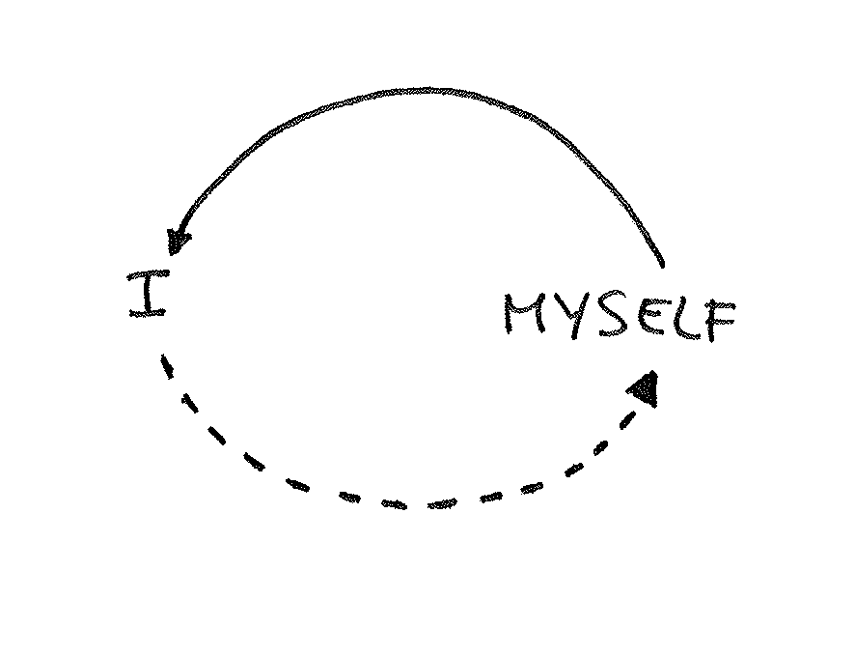
\includegraphics[width=1\linewidth]{L6-3b.png}
                    \captionof{figure}{Self-love as the pleasure of self-approval}
                \end{center}
            \end{minipage}


\newpage
        \subsubsection{The faculty of speech}

            \begin{figure}[h]
                \centering
                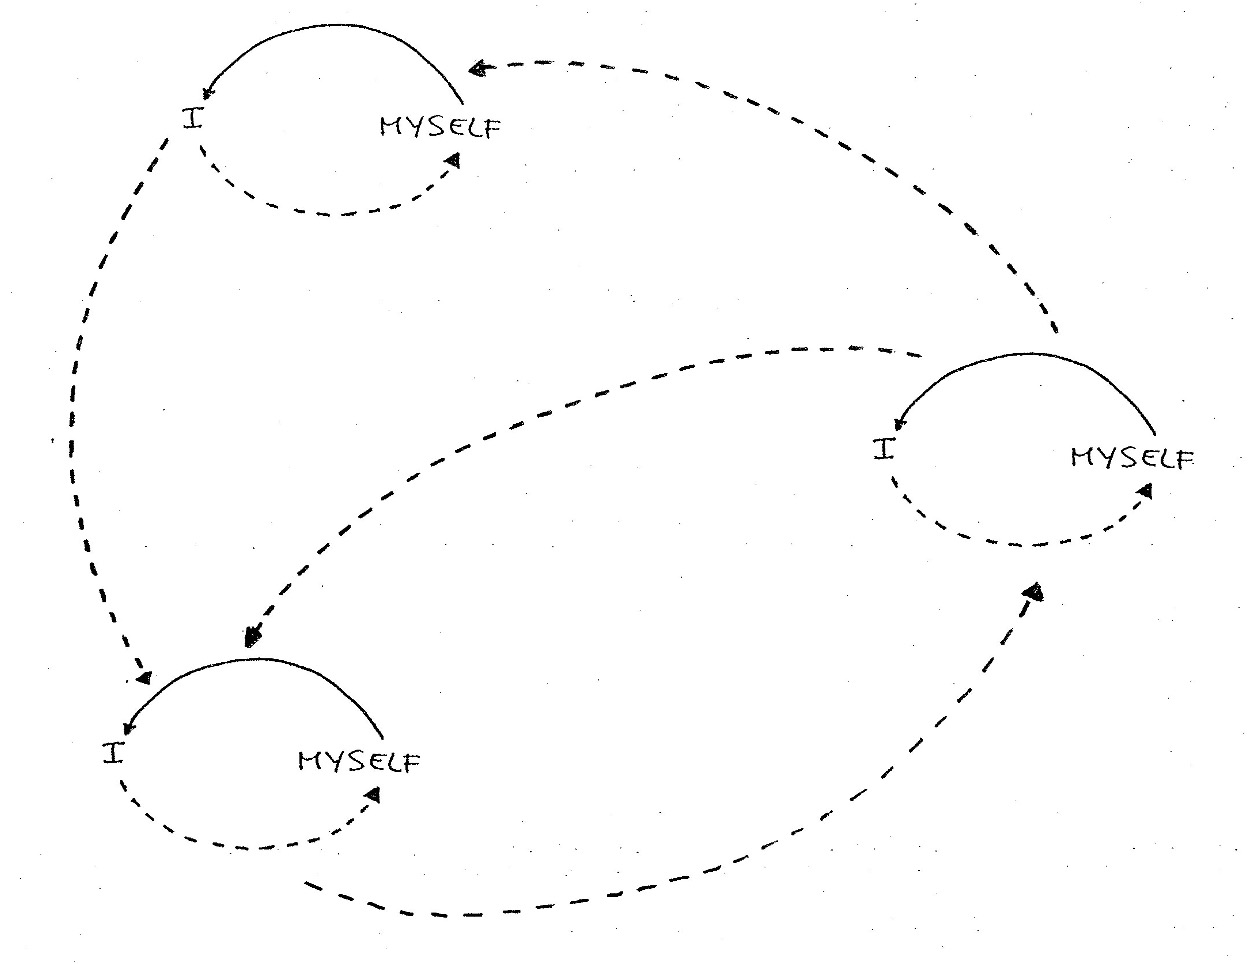
\includegraphics[width=0.5\linewidth]{L6-4.jpeg}
                \caption{Self-love as the pleasure of  deserved approval}
                \label{fig:enter-label}
            \end{figure}

            \begin{quote}
                Whether this propensity be one of those original principles in human nature, of which no further account can be given; or whether, as seems more probable, it be the necessary consequence of the faculties of reason and speech, it belongs not to our present subject to enquire. It is common to all men, and to be found in no other race of animals, which seem to know neither this nor any other species of contracts.
                
                Nobody ever saw a dog make a fair and deliberate exchange of one bone for another with another dog. Nobody ever saw one animal by its gestures and natural cries signify to another, this is mine, that yours; I am willing to give this for that. When an animal wants to obtain something…
            \end{quote}

            \begin{proposition}
                \textbf{The pleasure of exchange:} Adam Smith’s third kind of self-love
            \end{proposition}

\section[The Pleasure of Exchange]{The pleasure of exchange: Adam Smith’s third kind of self-love}

    \textbf{Question}: How to apply this third kind of Self-love to exchange?

    The butcher and all other professionals find confirmation of their self-esteem in the appreciation of their work. They continue their activities only if they receive this kind of confirmation.
        
    \begin{itemize}
        \item The person who sells apples downtown collects them in the countryside. He will continue to do so as long as buyers appreciate his efforts and validate his work by paying the agreed-upon price for the apples.
        \item The fact that buyers pay that price indicates that they appreciate the seller’s work; this recognition encourages him to keep selling apples.
    \end{itemize} 
        
    \textbf{The recognition is reciprocal}: if I’m not sure the other is really appreciating what I’m doing (or appreciating my goods), this will not satisfy my self-esteem, and I’ll stop selling them.
    \begin{itemize}
        \item \textbf{Third element in exchange}: recognition of self-estimate.
            \begin{itemize}
                \item[\(\Rightarrow\)] Through the \textbf{equivalence} (paying what the seller propose me to pay) we have the recognition. 
            \end{itemize}
        \end{itemize}

    \begin{remark}
        \begin{itemize}
            \item In a situation where there is a monopoly, where prices are imposed, exchange does not have this mutual recognition, and so there is no morality. This happens when there is no power bargain.
            \item Now, we’re out of the scheme of \textit{non-tuism}; I really have in mind the interest of the other in exchange, and I want the other’s satisfaction, which for me lead to my self-esteem. In Smith, it’s not a \textit{do-ut-des} situation as exchange is usually explained.
                \begin{itemize}
                    \item I accept what you give to me in order to continue to give to you. \textit{E.g., I do not do the professor because it gives me a decent salary, but I accept it because it allows me to do the professor and so to do the things that I like}.
                    \item It is not a tug of war. The price is not a way to obtain the maximum profit from both sides and then they eventually agree on a cut in the middle to unlock the situation. Instead, they both look for the price that makes them happy given the value that they convey to that good/service. 
                \end{itemize}
        \end{itemize}
    \end{remark}

    \begin{remark}
        \textbf{So, are we in a society where exchange has this morality?} Smith says, not really. Mercantilists do not care about it, they look for have monopolies, for example.
            \begin{itemize}
                \item According to Smith, this happens in a stationary society, while in a progressive society, workers start to be in a better situation with their master (in terms of bargaining power) and therefore everything improves.
            \end{itemize}
    \end{remark}

        \subsubsection{In the ‘early state’ of society}

            \begin{quote}
                In that early and rude state of society which precedes both the accumulation of stock and the appropriation of land, the proportion between the quantities of labour necessary for acquiring different objects seems to be the only circumstance which can afford any rule for exchanging them for one another. If among a nation of hunters, for example, it usually costs twice the labour to kill a beaver which it does to kill a deer, one beaver should naturally exchange for or be worth two deer. It is natural that what is usually the produce of two days or two hours labour, should be worth double of what is usually the produce of one day’s or one hour’s labour.
    
                (\textit{The Wealth of Nations}, I.VI)
            \end{quote} 

            2 hours \(\rightarrow\) beaver, 1 hour \(\rightarrow\) deer. So, 1 beaver = 2 deer. Thomas Aquinas talked about amount of labour as the value of exchange, but we also mentioned the value of exchange through Aristotle. There is a conflict.
    
            \begin{quote}
                If the one species of labour should be more severe than the other, some allowance will naturally be made for this superior hardship; and the produce of one hour’s labour in the one way may frequently exchange for that of two hours labour in the other. Or if the one species of labour requires an uncommon degree of dexterity and ingenuity, the esteem which men have for such talents, will naturally give a value to their produce, superior to what would be due to the time employed about it. Such talents can seldom be acquired but in consequence of long application, and the superior value of their produce may frequently be no more than a reasonable compensation for the time and labour which must be spent in acquiring them.
    
                (\textit{The Wealth of Nations}, I.VI)
            \end{quote}

            The point is that there is some quality that must be evaluated in the quantity of labour, and we must agree on its value. So, hardship and ingenuity must be evaluated.

        \subsubsection{Hardship and ingenuity}

            \begin{quote}
                It is often difficult to ascertain the proportion between two different quantities of labour. The time spent in two different sorts of work will not always alone determine this proportion. The different degrees of hardship endured, and of ingenuity exercised, must likewise be taken into account. There may be more labour in an hour’s hard work than in two hours easy business; or in an hour’s application to a trade which it cost ten years labour to learn, than in a month’s industry at an ordinary and obvious employment.

                (\textit{The Wealth of Nations}, I.V)
            \end{quote}

            \begin{remark}
                There may be more labour in 1 hour of hard work than in 2 hours of easy business. So, I cannot exchange with the previous proportion, which is static and myopic. 
            \end{remark}

        \subsubsection{In the ‘advanced state’ of society}

            \begin{quote}
                In the advanced state of society, allowances of this kind, for superior hardship and superior skill, are commonly made in the wages of labour; and something of the same kind must probably have taken place in its earliest and rudest period.

                (\textit{The Wealth of Nations}, I.VI)
            \end{quote} 

    \subsection{A contraposition of theories of value}

        \subsubsection{Aquinas’ theory of value}

            \begin{quote}
                If a farmer gave a bushel of wheat for a sandal, he would have an excess of labor in his product (“superabundantiam laboris in opere”) and would have also an excess of presents (“superabundantiam doni”) because he would be giving more than he would receive. But when all have what is theirs, they are in this way equal and do business with one another because the equality previously mentioned is possible for them.

                (\textit{Summa Theologiae})
            \end{quote}

        \subsubsection{Smith’s theory of value}

            \begin{quote}
                Exchanged goods “contain the value of a certain quantity of labour which we exchange for what is supposed at the time to contain the value of an equal quantity”.

                (\textit{The Wealth of Nations}, I.V)
            \end{quote} 

        \subsubsection{Back to "Hardship and ingenuity"}

            \begin{quote}
                But it is not easy to find any accurate measure either of hardship or ingenuity. In exchanging indeed the different productions of different sorts of labour for one another, some allowance is commonly made for both. It is adjusted, however, not by any accurate measure, but by the higgling and bargaining of the market, according to that sort of rough equality which, though not exact, is sufficient for carrying on the business of common life.

                (\textit{The Wealth of Nations}, I.V)
            \end{quote}

            \begin{remark}
                I recognise your hardship and my ingenuity by exchanging, otherwise it does not exist. So, it happens only in the negotiation.
            \end{remark}

\section*{Additional Context and Observations}

    \begin{remark}
        Both \textit{The Wealth of Nations} and \textit{The Theory of Moral Sentiments} are best understood in the context of the Enlightenment. Smith’s work not only laid the groundwork for modern economics but also provided deep insights into human behavior, ethics, and the emergence of social institutions.
    \end{remark}

    \begin{remark}
        The juxtaposition of economic self-interest and moral sentiment is central to Smith’s philosophy. While self-interest drives market activity, the capacity for sympathy and the internal judgment of the impartial spectator help maintain social order and ethical behavior.
    \end{remark}

    \begin{remark}
        The recurring theme of self-interest—whether expressed as the invisible hand in market transactions or as the pursuit of self-approval in moral judgment—suggests that human behavior, though seemingly divided between economic and moral spheres, is underpinned by a consistent set of motivations
    \end{remark}

    \begin{remark}
        Smith’s observations about the division of labour and market size illustrate that economic specialization is both enabled and limited by the structure of society. Similarly, the development of moral sentiments is linked to the unique human capacity for language and reflection.
    \end{remark}